\chapter{Verkkojen perusteet}

Voimme ratkaista monia algoritmisia ongelmia
esittämällä tilanteen \emph{verkkona} ja käyttämällä sitten
sopivaa verkkoalgoritmia.
Tyypillinen esimerkki verkosta on tieverkosto,
joka muodostuu kaupungeista ja niiden välisistä teistä.
Tällaisessa verkossa yksi luonteva kysymys on,
mitä reittiä pitkin voimme matkustaa kaupungista $a$ kaupunkiin $b$.

Tässä luvussa opimme ensin joitain verkkoihin liittyviä
peruskäsitteitä sekä tavan käsitellä verkkoja ohjelmoinnissa.
Tämän jälkeen tutustumme kahteen ensimmäiseen verkkoalgoritmiin:
syvyyshakuun ja leveyshakuun.
Jatkamme verkkojen käsittelyä kirjan seuraavissa luvuissa.

\section{Verkon esittäminen}

Verkko muodostuu \emph{solmuista} ja
niitä yhdistävistä \emph{kaarista}.
Sanomme, että kaksi solmua ovat \emph{vierekkäin} verkossa,
jos niiden välillä on kaari.
Solmun \emph{naapureja} ovat kaikki solmut,
joihin se on yhteydessä kaarella,
ja solmun \emph{aste} on sen naapureiden määrä.
Verkossa oleva \emph{polku} tarkoittaa reittiä
tietystä solmusta toiseen kulkemalla kaaria pitkin.

\begin{figure}
\center
\begin{center}
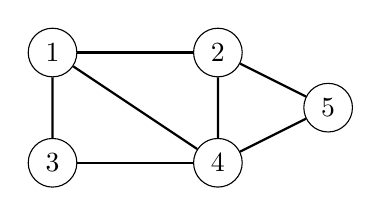
\begin{tikzpicture}[scale=0.7]
\node[draw, circle] (1) at (1,3) {$1$};
\node[draw, circle] (2) at (4,3) {$2$};
\node[draw, circle] (3) at (1,1) {$3$};
\node[draw, circle] (4) at (4,1) {$4$};
\node[draw, circle] (5) at (6,2) {$5$};

\path[draw,thick,-] (1) -- (2);
\path[draw,thick,-] (1) -- (3);
\path[draw,thick,-] (1) -- (4);
\path[draw,thick,-] (3) -- (4);
\path[draw,thick,-] (2) -- (4);
\path[draw,thick,-] (2) -- (5);
\path[draw,thick,-] (4) -- (5);
\end{tikzpicture}
\end{center}
\caption{Verkko, jossa on 5 solmua ja 7 kaarta.}
\label{fig:veresi}
\end{figure}

Merkitsemme tässä kirjassa verkon solmujen
määrää kirjaimella $n$ ja kaarten määrää
kirjaimella $m$.
Lisäksi numeroimme verkon solmut kokonaisluvuin
$1,2,\dots,n$.
Esimerkiksi kuvassa \ref{fig:veresi} on verkko,
jossa on 5 solmua ja 7 kaarta.
Solmun 2 naapurit ovat 1, 4 ja 5,
joten solmun aste on 3.
Voimme kulkea solmusta 1 solmuun 5
esimerkiksi polkua $1 \rightarrow 2 \rightarrow 5$
tai $1 \rightarrow 3 \rightarrow 4 \rightarrow 5$.

Matematiikassa verkko esitetään usein joukkoina $V$ ja $E$,
jotka ilmaisevat verkon solmut ja kaaret.
Nämä tulevat englannin kielen sanoista \emph{vertex} (solmu)
ja \emph{edge} (kaari).
Esimerkkiverkossamme
\[ V = \{1,2,3,4,5\} \]
ja
\[ E = \{\{1,2\},\{1,3\},\{1,4\},\{2,4\},\{2,5\},\{3,4\},\{4,5\} \}.\]
Huomaa, että tässä esityksessä kunkin kahden solmun välillä
voi olla enintään yksi kaari, mikä on yleensä luonteva rajoitus.

Ohjelmoinnissa tavallinen tapa esittää verkko on
luoda kullekin verkon solmulle \emph{vieruslista},
joka kertoo, mihin solmuihin voimme siirtyä solmusta kaarta pitkin.
Esimerkiksi Javassa voimme luoda taulukon

\begin{code}
ArrayList<Integer>[] verkko = new ArrayList<>[n+1];
\end{code}

ja alustaa vieruslistat näin:

\begin{code}
for (int i = 1; i <= n; i++) {
    verkko[i] = new ArrayList<>();
}
\end{code}

Tämän jälkeen voimme rakentaa esimerkkiverkkomme näin:

\begin{code}
verkko[1].add(2);
verkko[1].add(3);
verkko[1].add(4);
verkko[2].add(1);
verkko[2].add(4);
verkko[2].add(5);
verkko[3].add(1);
verkko[3].add(4);
verkko[4].add(1);
verkko[4].add(2);
verkko[4].add(3);
verkko[4].add(5);
verkko[5].add(2);
verkko[5].add(4);
\end{code}

\section{Syvyyshaku}

\emph{Syvyyshaku} on verkkojen käsittelyn perusalgoritmi,
joka etsii kaikki solmut, jotka ovat saavutettavissa
annetusta lähtösolmusta.
Voimme selvittää syvyyshaun avulla monia asioita
verkon rakenteesta.

Syvyyshaku lähtee liikkeelle tietystä verkon solmusta ja siirtyy
joka askeleella johonkin vielä tutkimattomaan solmuun,
johon nykyisestä solmusta pääsee kaarta pitkin.
Kuitenkin jos mitään tällaista solmua ei ole olemassa,
haku palaa takaisin kulkemallaan reitillä.

\begin{figure}
\center
\begin{center}
\begin{tikzpicture}[scale=0.6]
\scriptsize
\newcommand\verkko[6]{
\node[draw, circle, fill=#2] (1) at (0,0) {$1$};
\node[draw, circle, fill=#3] (2) at (2,0) {$2$};
\node[draw, circle, fill=#4] (3) at (0,-2) {$3$};
\node[draw, circle, fill=#5] (4) at (2,-2) {$4$};
\node[draw, circle, fill=#6] (5) at (4,-1) {$5$};
\path[draw,thick,-] (1) -- (2);
\path[draw,thick,-] (2) -- (5);
\path[draw,thick,-] (2) -- (4);
\path[draw,thick,-] (4) -- (5);
\path[draw,thick,-] (1) -- (3);
\node at (2,-3) {vaihe #1};
}
\begin{scope}
\verkko{1}{lightgray}{white}{white}{white}{white}
\end{scope}
\begin{scope}[xshift=6cm]
\verkko{2}{lightgray}{lightgray}{white}{white}{white}
\path[draw=red,thick,->,line width=2pt] (1) -- (2);
\end{scope}
\begin{scope}[xshift=12cm]
\verkko{3}{lightgray}{lightgray}{white}{lightgray}{white}
\path[draw=red,thick,->,line width=2pt] (1) -- (2);
\path[draw=red,thick,->,line width=2pt] (2) -- (4);
\end{scope}
\begin{scope}[xshift=18cm]
\verkko{4}{lightgray}{lightgray}{white}{lightgray}{lightgray}
\path[draw=red,thick,->,line width=2pt] (1) -- (2);
\path[draw=red,thick,->,line width=2pt] (2) -- (4);
\path[draw=red,thick,->,line width=2pt] (4) -- (5);
\end{scope}
\begin{scope}[yshift=-5cm]
\verkko{5}{lightgray}{lightgray}{white}{lightgray}{lightgray}
\path[draw=red,thick,->,line width=2pt] (1) -- (2);
\path[draw=red,thick,->,line width=2pt] (2) -- (4);
\path[draw=red,thick,->,line width=2pt] (4) -- (5);
\path[draw=red,thick,->,line width=2pt] (5) -- (2);
\end{scope}
\begin{scope}[yshift=-5cm,xshift=6cm]
\verkko{6}{lightgray}{lightgray}{white}{lightgray}{lightgray}
\path[draw=red,thick,->,line width=2pt] (1) -- (2);
\path[draw=red,thick,->,line width=2pt] (2) -- (4);
\path[draw=red,thick,->,line width=2pt] (4) -- (5);
\end{scope}
\begin{scope}[yshift=-5cm,xshift=12cm]
\verkko{7}{lightgray}{lightgray}{white}{lightgray}{lightgray}
\path[draw=red,thick,->,line width=2pt] (1) -- (2);
\path[draw=red,thick,->,line width=2pt] (2) -- (4);
\end{scope}
\begin{scope}[yshift=-5cm,xshift=18cm]
\verkko{8}{lightgray}{lightgray}{white}{lightgray}{lightgray}
\path[draw=red,thick,->,line width=2pt] (1) -- (2);
\end{scope}
\begin{scope}[yshift=-10cm]
\verkko{9}{lightgray}{lightgray}{white}{lightgray}{lightgray}
\end{scope}
\begin{scope}[yshift=-10cm,xshift=6cm]
\verkko{10}{lightgray}{lightgray}{lightgray}{lightgray}{lightgray}
\path[draw=red,thick,->,line width=2pt] (1) -- (3);
\end{scope}
\begin{scope}[yshift=-10cm,xshift=12cm]
\verkko{11}{lightgray}{lightgray}{lightgray}{lightgray}{lightgray}
\end{scope}
\end{tikzpicture}
\end{center}
\caption{Esimerkki syvyyshaun toiminnasta.}
\label{fig:syvhak}
\end{figure}

Kuvassa \ref{fig:syvhak} on esimerkki syvyyshaun toiminnasta.
Jokaisessa vaiheessa harmaat solmut ovat solmuja,
joissa haku on jo vieraillut.
Haku lähtee liikkeelle solmusta 1 ja etenee ensin
solmuihin 2, 4 ja 5.
Tämän jälkeen haku palaa takaisin solmuun 1
ja käy vielä solmussa 3.

\subsection{Algoritmin toteutus}

Syvyyshaku on mukavaa toteuttaa rekursiivisesti.
Tarvitsemme ensinnäkin taulukon, joka kertoo,
missä solmuissa olemme käyneet:

\begin{code}
boolean[] vierailtu = new boolean[n+1];
\end{code}

Tämän jälkeen voimme toteuttaa syvyyshaun näin:

\begin{code}
void syvyyshaku(int solmu) {
    if (vierailtu[solmu]) return;
    vierailtu[solmu] = true;
    for (Integer naapuri : verkko[solmu]) {
        syvyyshaku(naapuri);
    }
}
\end{code}

Syvyyshaku käynnistyy, kun kutsumme metodia
\texttt{syvyyshaku} parametrina lähtösolmu.
Jokaisella kutsulla metodi tarkistaa ensin,
olemmeko jo käyneet parametrina annetussa solmussa,
ja päättyy heti tässä tilanteessa.
Muuten metodi merkitsee, että olemme nyt käyneet solmussa
ja etenee rekursiivisesti kaikkiin solmun naapureihin.

Syvyyshaku vie aikaa $O(n+m)$, missä $n$ on solmujen määrä
ja $m$ on kaarten määrä,
koska käymme läpi kerran jokaisesta solmusta lähtevät kaaret.

\subsection{Sovelluksia}

\begin{figure}
\center
\begin{center}
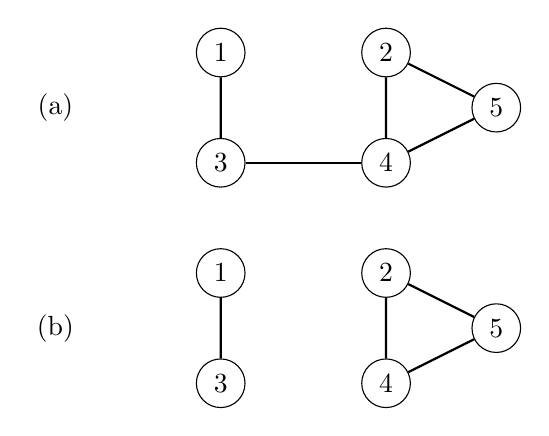
\begin{tikzpicture}[scale=0.7]
\begin{scope}
\node[draw, circle] (1) at (1,3) {$1$};
\node[draw, circle] (2) at (4,3) {$2$};
\node[draw, circle] (3) at (1,1) {$3$};
\node[draw, circle] (4) at (4,1) {$4$};
\node[draw, circle] (5) at (6,2) {$5$};
\path[draw,thick,-] (1) -- (3);
\path[draw,thick,-] (3) -- (4);
\path[draw,thick,-] (2) -- (4);
\path[draw,thick,-] (2) -- (5);
\path[draw,thick,-] (4) -- (5);
\node at (-2,2) {(a)};
\end{scope}
\begin{scope}[yshift=-4cm]
\node[draw, circle] (1) at (1,3) {$1$};
\node[draw, circle] (2) at (4,3) {$2$};
\node[draw, circle] (3) at (1,1) {$3$};
\node[draw, circle] (4) at (4,1) {$4$};
\node[draw, circle] (5) at (6,2) {$5$};
\path[draw,thick,-] (1) -- (3);
\path[draw,thick,-] (2) -- (4);
\path[draw,thick,-] (2) -- (5);
\path[draw,thick,-] (4) -- (5);
\node at (-2,2) {(b)};
\end{scope}
\end{tikzpicture}
\end{center}
\caption{(a) Verkko on yhtenäinen. (b) Verkon yhtenäiset komponentit ovat $\{1,3\}$ ja $\{2,4,5\}$.}
\label{fig:veryht}
\end{figure}

Kun suoritamme verkossa syvyyshaun tietystä solmusta alkaen,
löydämme polut kaikkiin solmuihin, joihin kyseisestä
solmusta pääsee.
Esimerkiksi kuvan \ref{fig:syvhak} syvyyshaun aikana
olemme saaneet selville polut solmusta 1 kaikkiin muihin solmuihin.
Tässä tapauksessa esimerkiksi polku solmusta $1$ solmuun $5$ on
$1 \rightarrow 2 \rightarrow 4 \rightarrow 5$,
joka on löytynyt haun vaiheessa 4.

Sanomme, että verkko on \emph{yhtenäinen},
jos verkossa on polku minkä tahansa kahden solmun välillä.
Verkko on yhtenäinen tarkalleen silloin,
kun pääsemme \emph{mistä tahansa} solmusta
kaikkiin muihin solmuihin.
Niinpä voimme tarkastaa yhtenäisyyden suorittamalla
syvyyshaun mielivaltaisesta solmusta alkaen.
Esimerkiksi kuvan \ref{fig:veryht}(a) verkko on yhtenäinen,
koska solmusta 1 alkava syvyyshaku käy kaikissa solmuissa.

Jos verkko ei ole yhtenäinen, se jakautuu
yhtenäisiin \emph{komponentteihin},
joista jokainen sisältää solmut, jotka ovat yhteydessä
toisiinsa.
Esimerkiksi kuvan \ref{fig:veryht}(b) verkon
yhtenäiset komponentit ovat $\{1,3\}$ ja $\{2,4,5\}$.
Löydäm\-me verkon yhtenäiset komponentit
käymällä läpi kaikki verkon solmut ja aloittamalla
uuden syvyyshaun aina, kun emme ole käyneet solmussa aiemmin.
Jokainen syvyyshaku löytää yhden yhtenäisen komponentin.

\section{Leveyshaku}

\emph{Leveyshaku} käy läpi solmuja lähtösolmusta aloittaen
järjestyksessä niiden etäisyyden mukaan.
Etäisyys solmuun tarkoittaa, kuinka pitkä on lyhin polku
lähtösolmusta solmuun.
Leveyshaun avulla voimmekin selvittää lyhimmän polun
pituuden lähtösolmusta muihin solmuihin.

\begin{figure}
\center
\begin{center}
\begin{tikzpicture}[scale=0.6]
\scriptsize
\newcommand\verkko[6]{
\node[draw, circle, fill=#2] (1) at (0,0) {$1$};
\node[draw, circle, fill=#3] (2) at (2,0) {$2$};
\node[draw, circle, fill=#4] (3) at (0,-2) {$3$};
\node[draw, circle, fill=#5] (4) at (2,-2) {$4$};
\node[draw, circle, fill=#6] (5) at (4,-1) {$5$};
\path[draw,thick,-] (1) -- (2);
\path[draw,thick,-] (2) -- (5);
\path[draw,thick,-] (2) -- (4);
\path[draw,thick,-] (4) -- (5);
\path[draw,thick,-] (1) -- (3);
\node at (2,-3) {vaihe #1};
}
\begin{scope}
\verkko{1}{lightgray}{white}{white}{white}{white}
\end{scope}
\begin{scope}[xshift=6cm]
\verkko{2}{lightgray}{lightgray}{white}{white}{white}
\path[draw=red,thick,->,line width=2pt] (1) -- (2);
\end{scope}
\begin{scope}[xshift=12cm]
\verkko{3}{lightgray}{lightgray}{lightgray}{white}{white}
\path[draw=red,thick,->,line width=2pt] (1) -- (3);
\end{scope}
\begin{scope}[xshift=18cm]
\verkko{4}{lightgray}{lightgray}{lightgray}{white}{white}
\path[draw=red,thick,->,line width=2pt] (2) -- (1);
\end{scope}
\begin{scope}[yshift=-5cm,xshift=0cm]
\verkko{5}{lightgray}{lightgray}{lightgray}{lightgray}{white}
\path[draw=red,thick,->,line width=2pt] (2) -- (4);
\end{scope}
\begin{scope}[yshift=-5cm,xshift=6cm]
\verkko{6}{lightgray}{lightgray}{lightgray}{lightgray}{lightgray}
\path[draw=red,thick,->,line width=2pt] (2) -- (5);
\end{scope}
\begin{scope}[yshift=-5cm,xshift=12cm]
\verkko{7}{lightgray}{lightgray}{lightgray}{lightgray}{lightgray}
\path[draw=red,thick,->,line width=2pt] (3) -- (1);
\end{scope}
\begin{scope}[yshift=-5cm,xshift=18cm]
\verkko{8}{lightgray}{lightgray}{lightgray}{lightgray}{lightgray}
\path[draw=red,thick,->,line width=2pt] (4) -- (2);
\end{scope}
\begin{scope}[yshift=-10cm,xshift=0cm]
\verkko{9}{lightgray}{lightgray}{lightgray}{lightgray}{lightgray}
\path[draw=red,thick,->,line width=2pt] (4) -- (5);
\end{scope}
\begin{scope}[yshift=-10cm,xshift=6cm]
\verkko{10}{lightgray}{lightgray}{lightgray}{lightgray}{lightgray}
\path[draw=red,thick,->,line width=2pt] (5) -- (2);
\end{scope}
\begin{scope}[yshift=-10cm,xshift=12cm]
\verkko{11}{lightgray}{lightgray}{lightgray}{lightgray}{lightgray}
\path[draw=red,thick,->,line width=2pt] (5) -- (4);
\end{scope}
\end{tikzpicture}
\end{center}
\caption{Esimerkki leveyshaun toiminnasta.}
\label{fig:levhak}
\end{figure}

Kuvassa \ref{fig:levhak} on esimerkki leveyshaun toiminnasta.
Haku vierailee solmuissa järjestyksessä 1, 2, 3, 4, 5.
Tämän järjestyksen mukaisesti haku tarkistaa jokaisesta solmusta,
mihin solmuihin siitä voi päästä.
Etäisyys solmuihin 2 ja 3 on 1, ja etäisyys solmuihin 4 ja 5 on 2.

\subsection{Algoritmin toteuttaminen}

Leveyshaku on vaikeampi toteuttaa kuin syvyyshaku,
koska meidän täytyy pystyä edistämään hakua vuorotellen verkon eri puolilta.
Tätä varten määrit\-telemme jonon, joka sisältää solmuja,
jotka odottavat läpikäyntiä.
Valitsemme aina seuraavaksi käsiteltävän solmun jonon alusta,
ja lisämme uudet vieraillut solmut jonon loppuun.
Voimme luoda jonon näin:

\begin{code}
ArrayDeque<Integer> jono = new ArrayDeque<>();
\end{code}

Lisäksi määrittelemme taulukot, joissa pidämme kirjaa,
missä solmuissa olemme käyneet sekä mitkä ovat solmujen
etäisyydet lähtösolmusta:

\begin{code}
boolean[] vierailtu = new boolean[n+1];
int[] etaisyys = new int[n+1];
\end{code}

Nyt voimme toteuttaa leveyshaun seuraavasti solmusta \texttt{alku} lähtien:

\begin{code}
vierailtu[alku] = true;
jono.addLast(alku);
while (jono.size() > 0) {
    int solmu = jono.pollFirst();
    for (int naapuri : verkko[solmu]) {
        if (vierailtu[naapuri]) continue;
        vierailtu[naapuri] = true;
        jono.addLast(naapuri);
    }
}
\end{code}

Koodi merkitsee aluksi, että olemme käyneet lähtösolmussa
ja etäisyys siihen on 0, sekä lisää lähtösolmun jonoon.
Sen jälkeen niin kauan kuin jonossa on solmuja,
koodi valitsee aina jonon ensimmäisen solmun
ja tarkastaa siitä lähtevät kaaret.
Jos pääsemme uuteen solmuun, päivitämme taulukkoja
sen solmun osalta ja lisäämme sen jonoon.

Syvyyshaun tavoin leveyshaku vie aikaa $O(n+m)$,
koska käymme läpi kerran jokaisesta solmusta lähtevät kaaret.

\section{Esimerkki: Labyrintti}

\section{Esimerkki: Labyrintti}

Olemme labyrintissa ja haluamme päästä ruudusta $A$ ruutuun $B$.
Joka askeleella voimme siirtyä yhden ruudun verran ylöspäin, alaspäin,
vasemmalle tai oikealle.
Pystymmekö pääsemään ruudusta $A$ ruutuun $B$, ja jos pystymme, niin
mikä on lyhin mahdollinen reitti?

\begin{figure}
\center
\begin{center}
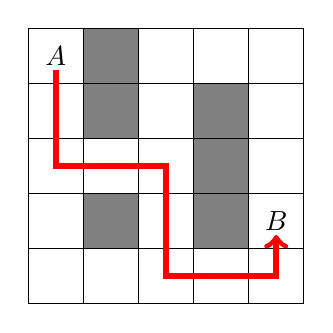
\begin{tikzpicture}[scale=0.7]
\draw[fill=gray] (1,1) rectangle (2,2);
\draw[fill=gray] (1,3) rectangle (2,4);
\draw[fill=gray] (1,4) rectangle (2,5);
\draw[fill=gray] (3,1) rectangle (4,2);
\draw[fill=gray] (3,2) rectangle (4,3);
\draw[fill=gray] (3,3) rectangle (4,4);
\draw (0,0) grid (5,5);
\draw[->,thick,red,line width=2pt] (0.5,4.25) -- (0.5,2.5) -- (2.5,2.5) -- (2.5,0.5) -- (4.5,0.5) -- (4.5,1.25);
\node at (0.5,4.5) {$A$};
\node at (4.5,1.5) {$B$};
\end{tikzpicture}
\end{center}
\caption{Lyhin reitti labyrintissa ruudusta $A$ ruutuun $B$.}
\label{fig:labrei}
\end{figure}

Esimerkiksi kuva \ref{fig:labrei} näyttää labyrintin, jossa lyhin reitti
ruudusta $A$ ruutuun $B$ muodostuu 9 askeleesta.

\begin{figure}
\center
\begin{center}
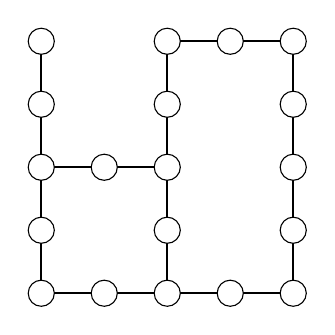
\begin{tikzpicture}[scale=0.8]
\foreach \x in {0,1,2,3} \path[draw,thick,-] (0,\x) -- (0,\x+1);
\foreach \x in {0,1,2,3} \path[draw,thick,-] (2,\x) -- (2,\x+1);
\foreach \x in {0,1,2,3} \path[draw,thick,-] (4,\x) -- (4,\x+1);
\foreach \x in {0,1,2,3} \path[draw,thick,-] (\x,0) -- (\x+1,0);
\foreach \x in {0,1} \path[draw,thick,-] (\x,2) -- (\x+1,2);
\foreach \x in {2,3} \path[draw,thick,-] (\x,4) -- (\x+1,4);
\foreach \x in {0,1,2,3,4} \node[draw, circle, fill=white] at (0,\x) {};
\foreach \x in {0,2} \node[draw, circle, fill=white] at (1,\x) {};
\foreach \x in {0,1,2,3,4} \node[draw, circle, fill=white] at (2,\x) {};
\foreach \x in {0,4} \node[draw, circle, fill=white] at (3,\x) {};
\foreach \x in {0,1,2,3,4} \node[draw, circle, fill=white] at (4,\x) {};
\end{tikzpicture}
\end{center}
\caption{Labyrintin esittäminen verkkona.}
\label{fig:labver}
\end{figure}

Voimme esittää tilanteen verkkona niin,
että jokainen labyrintin ruutu on yksi verkon solmuista,
ja kahden solmun välillä on kaari,
jos vastaavat ruudut ovat vierekkäin labyrintissa.
Kuva \ref{fig:labver} näyttää äskeistä esimerkkiä vastaavan
labyrintin verkkona.

Nyt meidän on helppoa selvittää, onko ruudusta $A$ reittiä
ruutuun $B$, koska näin on tarkalleen silloin,
jos vastaavat verkon solmut kuuluvat samaan komponenttiin.
Voimme tarkastaa tämän syvyyshaun avulla.
Jos haluamme lisäksi löytää lyhimmän reitin ruudusta $A$
ruutuun $B$, voimme puolestaan käyttää leveyshakua,
joka lähtee liikkeelle ruudusta $A$.

Huomaa, että meidän ei tarvitse erikseen muuttaa labyrinttia
verkoksi, vaan voimme toteuttaa haut \emph{implisiittiseen} verkkoon.
Tämä tarkoittaa, että teemme haun labyrinttiin sen omassa
esitystavassa. Käytännössä labyrintti on kätevää tallentaa kaksiulotteisena
taulukkona, joka ilmaisee, mitkä ruudut ovat lattiaa ja seinää.
Tällöin voimme toteuttaa esimerkiksi syvyyshaun seuraavan tyylisesti:

\begin{code}
void syvyyshaku(int y, int x) {
    if (y < 0 || x < 0 || y >= n || x >= n) return;
    if (seina[y][x] || vierailtu[y][x]) return;
    vierailtu[y][x] = true;
    syvyyshaku(y+1,x);
    syvyyshaku(y-1,x);
    syvyyshaku(y,x+1);
    syvyyshaku(y,x-1);
}
\end{code}

Haku haarautuu neljään suuntaan, koska voimme liikkua labyrintissa
ylöspäin, alaspäin, vasemmalle tai oikealle.
Emme kuitenkaan saa mennä labyrintin reunojen ulkopuolelle,
seinäruutuun tai ruutuun, jossa olemme käyneet jo aiemmin.


% \section{Verkkojen käsitteitä}
% 
% Verkko on tietorakenne, joka muodostuu \emph{solmuista} ja
% niitä yhdistävistä \emph{kaarista}.
% Merkitsemme tässä kirjassa verkon solmujen
% määrää kirjaimella $n$ ja kaarten määrää
% kirjaimella $m$.
% Lisäksi numeroimme verkon solmut kokonaisluvuin
% $1,2,\dots,n$.
% 
% Sanomme, että kaksi solmua ovat \emph{vierekkäin} verkossa,
% jos niiden välillä on kaari.
% Solmun \emph{naapureja} ovat kaikki solmut,
% joihin se on yhteydessä kaarella,
% ja solmun \emph{aste} on sen naapureiden määrä.
% Verkossa oleva \emph{polku} tarkoittaa reittiä
% tietystä solmusta toiseen kulkemalla kaaria pitkin.
% 
% Kuvassa \ref{fig:veresi} on esimerkkinä verkko,
% jossa on 5 solmua ja 7 kaarta.
% Solmun 2 aste on 3,
% koska sen naapurit ovat solmut 1, 4 ja 5.
% Voimme kulkea solmusta 1 solmuun 5 monella tavalla:
% mahdollisia polkuja ovat esimerkiksi
% $1 \rightarrow 2 \rightarrow 5$ ja
% $1 \rightarrow 3 \rightarrow 4 \rightarrow 5$.
% 
% 
% Verkko on \emph{yhtenäinen}, jos minkä tahansa
% kahden solmun välillä on polku.
% Esimerkiksi kuvan \ref{fig:veresi} verkko on yhtenäinen.
% Jos verkko ei ole yhtenäinen, voimme tarkastella
% sen yhtenäisiä \emph{komponentteja}.
% Esimerkiksi kuvan \ref{fig:veryht} verkko ei ole yhtenäinen,
% ja sen komponentit ovat $\{1,3\}$ ja $\{2,4,5\}$.
% 
% \begin{figure}
% \center
% \begin{center}
% \begin{tikzpicture}[scale=0.7]
% \node[draw, circle] (1) at (1,3) {$1$};
% \node[draw, circle] (2) at (4,3) {$2$};
% \node[draw, circle] (3) at (1,1) {$3$};
% \node[draw, circle] (4) at (4,1) {$4$};
% \node[draw, circle] (5) at (6,2) {$5$};
% 
% \path[draw,thick,-] (1) -- (3);
% \path[draw,thick,-] (2) -- (4);
% \path[draw,thick,-] (2) -- (5);
% \path[draw,thick,-] (4) -- (5);
% \end{tikzpicture}
% \end{center}
% \caption{Verkon yhtenäiset komponentit ovat $\{1,3\}$ ja $\{2,4,5\}$.}
% \label{fig:veryht}
% \end{figure}
% 
% Verkossa oleva \emph{sykli} on polku, jonka ensimmäinen ja viimeinen
% solmu on sama.
% Esimerkiksi verkossa \ref{fig:veresi} on sykli
% $1 \rightarrow 4 \rightarrow 3 \rightarrow 1$.
% Verkko on \emph{syklitön}, jos siinä ei ole yhtään sykliä.
% Verkko on \emph{puu}, jos se on yhtenäinen ja syklitön.
% Puussa kaarten määrä on aina yhden pienempi kuin solmujen määrä,
% ja jokaisen kahden solmun välillä on yksikäsitteinen polku.
% Esimerkiksi kuvassa \ref{fig:verpuu} on puu, jossa on 5 solmua ja 4 kaarta.
% 
% \begin{figure}
% \center
% \begin{center}
% \begin{tikzpicture}[scale=0.7]
% \node[draw, circle] (1) at (1,3) {$1$};
% \node[draw, circle] (2) at (4,3) {$2$};
% \node[draw, circle] (3) at (1,1) {$3$};
% \node[draw, circle] (4) at (4,1) {$4$};
% \node[draw, circle] (5) at (6,2) {$5$};
% 
% \path[draw,thick,-] (1) -- (3);
% \path[draw,thick,-] (3) -- (4);
% \path[draw,thick,-] (2) -- (4);
% \path[draw,thick,-] (4) -- (5);
% \end{tikzpicture}
% \end{center}
% \caption{Puu, jossa on 5 solmua ja 4 kaarta.}
% \label{fig:verpuu}
% \end{figure}
% 
% Verkko on \emph{suunnattu}, jos kaarilla on merkityt suunnat,
% joiden mukaisesti niitä on kuljettava.
% Kaarten suunnat voivat aiheuttaa, että emme voi liikkua
% verkossa yhtä vapaasti kuin ennen.
% Kuvassa \ref{fig:versuu} on esimerkkinä suunnattu verkko,
% jossa voimme esimerkiksi kulkea solmusta 1 solmuun 5
% polkua $1 \rightarrow 2 \rightarrow 5$,
% mutta emme voi kulkea mitenkään solmusta 5 solmuun 1.
% 
% \begin{figure}
% \center
% \begin{center}
% \begin{tikzpicture}[scale=0.7]
% \node[draw, circle] (1) at (1,3) {$1$};
% \node[draw, circle] (2) at (4,3) {$2$};
% \node[draw, circle] (3) at (1,1) {$3$};
% \node[draw, circle] (4) at (4,1) {$4$};
% \node[draw, circle] (5) at (6,2) {$5$};
% 
% \path[draw,thick,->] (1) -- (2);
% \path[draw,thick,<-] (1) -- (3);
% \path[draw,thick,<-] (1) -- (4);
% \path[draw,thick,->] (3) -- (4);
% \path[draw,thick,->] (2) -- (4);
% \path[draw,thick,->] (2) -- (5);
% \path[draw,thick,->] (4) -- (5);
% \end{tikzpicture}
% \end{center}
% \caption{Suunnattu verkko.}
% \label{fig:versuu}
% \end{figure}
% 
% Suunnattu verkko on \emph{vahvasti yhtenäinen},
% jos verkossa on polku mistä tahansa solmusta
% mihin tahansa solmuun.
% Esimerkiksi kuvan \ref{fig:versuu} verkko ei
% ole vahvasti yhtenäinen,
% koska emme voi kulkea solmusta 5 solmuun 1.
% Jos verkko ei ole vahvasti yhtenäinen,
% voimme kuitenkin jakaa sen vahvasti yhtenäisiin komponentteihin.
% Esimerkiksi kuvan \ref{fig:versuu} verkossa
% vahvasti yhtenäiset komponentit ovat $\{1,2,4\}$, $\{3\}$ ja $\{5\}$.
% 
% Suunnatussa verkossa solmun \emph{lähtöaste} on
% solmusta lähtevien kaarten määrä ja solmun \emph{tuloaste}
% on solmuun tulevien kaarten määrä.
% Esimerkiksi kuvan \ref{fig:versuu} verkossa
% solmun 2 lähtöaste on 2, koska siitä lähtee kaaret solmuihin 4 ja 5,
% ja sen tuloaste on 1, koska siihen tulee kaari solmusta 1.
% 
% Verkko on \emph{painotettu}, jos sen kaarille on asetettu painot.
% Usein painot kuvaavat kaarten pituuksia, ja polun pituus
% on siinä olevien painojen summa.
% Kuvassa \ref{fig:verpai} on esimerkki painotetusta verkosta.
% Esimerkiksi polun $1 \rightarrow 2 \rightarrow 5$ pituus on $5+2=7$
% ja polun $1 \rightarrow 4 \rightarrow 5$ pituus on $1+3=4$.
% Tässä verkossa jälkimmäinen polku on \emph{lyhin polku} solmusta 1 solmuun 5.
% 
% \begin{figure}
% \center
% \begin{center}
% \begin{tikzpicture}[scale=0.7,label distance=-1.5mm]
% \node[draw, circle] (1) at (1,3) {$1$};
% \node[draw, circle] (2) at (4,3) {$2$};
% \node[draw, circle] (3) at (1,1) {$3$};
% \node[draw, circle] (4) at (4,1) {$4$};
% \node[draw, circle] (5) at (6,2) {$5$};
% 
% \path[draw,thick,-] (1) -- node[font=\small,label=above:5] {} (2);
% \path[draw,thick,-] (1) -- node[font=\small,label=left:2] {} (3);
% \path[draw,thick,-] (1) -- node[font=\small,label=above:1] {} (4);
% \path[draw,thick,-] (3) -- node[font=\small,label=below:4] {} (4);
% \path[draw,thick,-] (2) -- node[font=\small,label=right:7] {} (4);
% \path[draw,thick,-] (2) -- node[font=\small,label=above:2] {} (5);
% \path[draw,thick,-] (4) -- node[font=\small,label=below:3] {} (5);
% \end{tikzpicture}
% \end{center}
% \caption{Painotettu verkko.}
% \label{fig:verpai}
% \end{figure}
% 
% Verkko on \emph{kaksijakoinen}, jos voimme värittää sen
% solmut kahdella värillä niin, että jokaisella
% vierekkäisellä solmulla on eri väri.
% Esimerkiksi kuvan \ref{fig:verkak} verkko on kaksijakoinen,
% koska voimme värittää solmut 1 ja 4 sinisiksi ja
% solmut 2, 3 ja 5 punaisiksi.
% 
% \begin{figure}
% \center
% \begin{center}
% \begin{tikzpicture}[scale=0.7]
% \node[draw, circle, color=blue] (1) at (1,3) {$1$};
% \node[draw, circle, color=red] (2) at (4,3) {$2$};
% \node[draw, circle, color=red] (3) at (1,1) {$3$};
% \node[draw, circle, color=blue] (4) at (4,1) {$4$};
% \node[draw, circle, color=red] (5) at (6,2) {$5$};
% 
% \path[draw,thick,-] (1) -- (2);
% \path[draw,thick,-] (1) -- (3);
% \path[draw,thick,-] (3) -- (4);
% \path[draw,thick,-] (2) -- (4);
% \path[draw,thick,-] (4) -- (5);
% \end{tikzpicture}
% \end{center}
% \caption{Kaksijakoinen verkko, jossa voimme värittää solmut 1 ja 4
% sinisiksi ja solmut 2, 3 ja 5 punaisiksi.}
% \label{fig:verkak}
% \end{figure}
% 
% \section{Verkot ohjelmoinnissa}
% 
% Verkkojen käsittelyyn ohjelmoinnissa on monia tapoja.
% Seuraavaksi käymme läpi kolme tavallista esitystapaa,
% jotka tulevat myöhemmin käyttöön kirjan algoritmeissa.
% Jokaisessa tavassa on omat hyvät ja huonot puolensa.
% 
% \subsection{Vieruslistaesitys}
% 
% Verkon vieruslistaesityksessä jokaisella solmulla on
% \emph{vieruslista}, joka ilmaisee, mihin solmuihin
% solmusta lähtee kaari.
% Kuvassa \ref{fig:vervil} on esimerkkinä suunnattu verkko
% sekä sitä vastaava vieruslistaesitys.
% 
% \begin{figure}
% \center
% \begin{center}
% \begin{tikzpicture}[scale=0.7]
% \begin{scope}
% \node[draw, circle] (1) at (1,3) {$1$};
% \node[draw, circle] (2) at (4,3) {$2$};
% \node[draw, circle] (3) at (1,1) {$3$};
% \node[draw, circle] (4) at (4,1) {$4$};
% \node[draw, circle] (5) at (6,2) {$5$};
% 
% \path[draw,thick,->] (1) -- (2);
% \path[draw,thick,<-] (1) -- (3);
% \path[draw,thick,<-] (1) -- (4);
% \path[draw,thick,->] (3) -- (4);
% \path[draw,thick,->] (2) -- (4);
% \path[draw,thick,->] (2) -- (5);
% \path[draw,thick,->] (4) -- (5);
% \end{scope}
% \begin{scope}[scale=0.8,xshift=12cm,yshift=0.25cm]
% %\draw (0,0) grid (1,5);
% \draw (2,1) grid (3,5);
% \draw (4,1) grid (5,4);
% \foreach \y/\v in {0/1,1/2,2/3,3/4,4/5} \node at (0.5,4.5-\y) {\v};
% \draw (1,5) -- (1,0);
% \node at (2.5,4.5) {2};
% \node at (2.5,3.5) {4};
% \node at (4.5,3.5) {5};
% \node at (2.5,2.5) {1};
% \node at (4.5,2.5) {4};
% \node at (2.5,1.5) {1};
% \node at (4.5,1.5) {5};
% \path[draw,thick,->] (1.0,4.5) -- (2,4.5);
% \path[draw,thick,->] (1.0,3.5) -- (2,3.5);
% \path[draw,thick,->] (1.0,2.5) -- (2,2.5);
% \path[draw,thick,->] (1.0,1.5) -- (2,1.5);
% \path[draw,thick,->] (3,3.5) -- (4.0,3.5);
% \path[draw,thick,->] (3,2.5) -- (4.0,2.5);
% \path[draw,thick,->] (3,1.5) -- (4.0,1.5);
% \end{scope}
% \end{tikzpicture}
% \end{center}
% \caption{Verkon vieruslistaesitys.}
% \label{fig:vervil}
% \end{figure}
% 
% Javassa voimme tallentaa verkon vieruslistaesityksen
% taulukkona, jonka jokaisessa kohdassa on tietyn
% solmun vieruslista.
% Seuraava koodi määrittelee tällaisen taulukon:
% 
% \begin{code}
% ArrayList<Integer>[] verkko = new ArrayList<>[n+1];
% \end{code}
% 
% Ennen kuin voimme käyttää taulukkoa,
% meidän täytyy alustaa jokainen vieruslista:
% 
% \begin{code}
% for (int i = 1; i <= n; i++) {
%     verkko[i] = new ArrayList<>();
% }
% \end{code}
% 
% Tämän jälkeen voimme lisätä kaaret verkkoon näin:
% 
% \begin{code}
% verkko[1].add(2);
% verkko[2].add(4);
% verkko[2].add(5);
% verkko[3].add(1);
% verkko[3].add(4);
% verkko[4].add(1);
% verkko[4].add(5);
% \end{code}
% 
% Jos verkko on suuntaamaton, voimme menetellä muuten samoin,
% mutta tallennamme kunkin kaaren molempiin suuntiin.
% Jos taas verkko on painotettu, voimme tallentaa listaan
% olioita, joissa on kaaren kohdesolmu ja paino.
% Esimerkiksi voisimme käyttää seuraavanlaista luokkaa:
% 
% \begin{code}
% class Kaari {
%     int kohde, paino;
% 
%     public Kaari(int kohde, int paino) {
%         this.kohde = kohde;
%         this.paino = paino;
%     }
% }
% \end{code}
% 
% Vieruslistaesitys on yleensä käytännössä hyvä tapa
% tallentaa verkko ohjelmoinnissa.
% Esityksen avulla voimme selvittää helposti,
% mihin solmuihin pääsee kaarta pitkin tietystä solmusta.
% Esimerkiksi voimme käydä seuraavasti läpi
% kaikki tietyn solmun naapurit:
% 
% \begin{code}
% for (int naapuri : verkko[solmu]) {
%     // käsittele naapuri
% }
% \end{code}
% 
% \subsection{Vierusmatriisiesitys}
% 
% Verkon vierusmatriisi on $n \times n$ -kokoinen matriisi
% (eli kaksiulotteinen taulukko), joka kuvaa, mitä kaaria verkossa on.
% Matriisissa rivin $a$ sarakkeessa $b$ on luku 1,
% jos verkossa on kaari solmusta $a$ solmuun $b$,
% ja muuten luku 0.
% Kuvassa \ref{fig:vervim} on esimerkki verkon
% vierusmatriisiesityksestä.
% 
% \begin{figure}
% \center
% \begin{center}
% \begin{tikzpicture}[scale=0.7]
% \begin{scope}
% \node[draw, circle] (1) at (1,3) {$1$};
% \node[draw, circle] (2) at (4,3) {$2$};
% \node[draw, circle] (3) at (1,1) {$3$};
% \node[draw, circle] (4) at (4,1) {$4$};
% \node[draw, circle] (5) at (6,2) {$5$};
% 
% \path[draw,thick,->] (1) -- (2);
% \path[draw,thick,<-] (1) -- (3);
% \path[draw,thick,<-] (1) -- (4);
% \path[draw,thick,->] (3) -- (4);
% \path[draw,thick,->] (2) -- (4);
% \path[draw,thick,->] (2) -- (5);
% \path[draw,thick,->] (4) -- (5);
% \end{scope}
% \begin{scope}[scale=0.8,xshift=12cm,yshift=0.25cm]
% \draw (0,0) grid (5,5);
% \foreach \x in {1,2,3,4,5} \node at (-0.5,5.5-\x) {\x};
% \foreach \x in {1,2,3,4,5} \node at (-0.5+\x,5.5) {\x};
% 
% \foreach \x/\v in {1/0,2/1,3/0,4/0,5/0} \node at (-0.5+\x,4.5) {\v};
% \foreach \x/\v in {1/0,2/0,3/0,4/1,5/1} \node at (-0.5+\x,3.5) {\v};
% \foreach \x/\v in {1/1,2/0,3/0,4/1,5/0} \node at (-0.5+\x,2.5) {\v};
% \foreach \x/\v in {1/1,2/0,3/0,4/0,5/1} \node at (-0.5+\x,1.5) {\v};
% \foreach \x/\v in {1/0,2/0,3/0,4/0,5/0} \node at (-0.5+\x,0.5) {\v};
% \end{scope}
% \end{tikzpicture}
% \end{center}
% \caption{Verkon vierusmatriisiesitys.}
% \label{fig:vervim}
% \end{figure}
% 
% Javassa voimme määritellä vierusmatriisia varten seuraavanlaisen taulukon:
% 
% \begin{code}
% int[][] verkko = new int[n+1][n+1];
% \end{code}
% 
% Tämän jälkeen voimme lisätä kaaret matriisiin näin:
% 
% \begin{code}
% verkko[1][2] = 1;
% verkko[2][4] = 1;
% verkko[2][5] = 1;
% verkko[3][1] = 1;
% verkko[3][4] = 1;
% verkko[4][1] = 1;
% verkko[4][5] = 1;
% \end{code}
% 
% Jos verkko on painotettu, voimme merkitä matriisiin luvun 1 sijasta
% kunkin kaaren painon.
% 
% Vierusmatriisiesityksen etuna on, että voimme tarkistaa tehokkaasti,
% onko jokin tietty kaari verkossa.
% Huonona puolena on kuitenkin, että esitystapa vie paljon tilaa:
% kun verkossa on $n$ kaarta, vierusmatriisi varten tarvitaan taulukko,
% jossa on $O(n^2)$ alkiota.
% Usein verkossa on vain pieni osa mahdollisista kaarista,
% jolloin vierusmatriisiesitys tuhlaa muistia.
% 
% \subsection{Kaarilistaesitys}
% 
% Verkon kaarilistaesityksessä tallennamme listan,
% jonka jokainen alkio on yksi verkon kaarista.
% Kuva \ref{fig:verkal} näyttää esimerkin kaarilistaesityksestä.
% 
% \begin{figure}
% \center
% \begin{center}
% \begin{tikzpicture}[scale=0.7]
% \begin{scope}
% \node[draw, circle] (1) at (1,3) {$1$};
% \node[draw, circle] (2) at (4,3) {$2$};
% \node[draw, circle] (3) at (1,1) {$3$};
% \node[draw, circle] (4) at (4,1) {$4$};
% \node[draw, circle] (5) at (6,2) {$5$};
% 
% \path[draw,thick,->] (1) -- (2);
% \path[draw,thick,<-] (1) -- (3);
% \path[draw,thick,<-] (1) -- (4);
% \path[draw,thick,->] (3) -- (4);
% \path[draw,thick,->] (2) -- (4);
% \path[draw,thick,->] (2) -- (5);
% \path[draw,thick,->] (4) -- (5);
% \end{scope}
% \begin{scope}[scale=0.8,xshift=0cm,yshift=-1.5cm]
% \node[draw, rectangle] (1) at (0,0) {$(1,2)$};
% \node[draw, rectangle] (2) at (3,0) {$(2,4)$};
% \node[draw, rectangle] (3) at (6,0) {$(2,5)$};
% \node[draw, rectangle] (4) at (9,0) {$(3,1)$};
% \node[draw, rectangle] (5) at (12,0) {$(3,4)$};
% \node[draw, rectangle] (6) at (15,0) {$(4,1)$};
% \node[draw, rectangle] (7) at (18,0) {$(4,5)$};
% \path[draw,thick,->] (1) -- (2);
% \path[draw,thick,->] (2) -- (3);
% \path[draw,thick,->] (3) -- (4);
% \path[draw,thick,->] (4) -- (5);
% \path[draw,thick,->] (5) -- (6);
% \path[draw,thick,->] (6) -- (7);
% \end{scope}
% \end{tikzpicture}
% \end{center}
% \caption{Verkon kaarilistaesitys.}
% \label{fig:verkal}
% \end{figure}
% 
% Kaaria varten voimme luoda seuraavanlaisen luokan:
% 
% \begin{code}
% class Kaari {
%     public int alku, loppu;
% 
%     public Kaari(int alku, int loppu) {
%         this.alku = alku;
%         this.loppu = loppu;
%     }
% }
% \end{code}
% 
% Tämän jälkeen voimme muodostaa listan seuraavasti:
% 
% \begin{code}
% ArrayList<Kaari> kaaret = new ArrayList<>();
% kaaret.add(new Kaari(1,2));
% kaaret.add(new Kaari(2,4));
% kaaret.add(new Kaari(2,5));
% kaaret.add(new Kaari(3,1));
% kaaret.add(new Kaari(3,4));
% kaaret.add(new Kaari(4,1));
% kaaret.add(new Kaari(4,5));
% \end{code}
% 
% Jos kaarilla on painot, voimme lisätä luokkaan yhden kentän lisää,
% johon tallennetaan kaaren paino.
% 
% Kaarilistaesitys on kätevä silloin, jos algoritmin tulee käydä
% kaikki verkon kaaret läpi, koska silloin riittää tehdä yksi
% for-silmukka, joka käy listan läpi:
% 
% \begin{code}
% for (Kaari kaari : kaaret) {
%     // käsittele kaari
% }
% \end{code}
% 
% Esityksen huonona puolena on, että listalta on hidasta etsiä tietystä
% solmusta lähtevät kaaret.
